% Paquets généraux
\documentclass[a4paper,12pt,titlepage,twoside]{article}
\usepackage[utf8]{inputenc}
\usepackage[T1]{fontenc}
\usepackage[french]{babel}
\usepackage{textgreek}
\usepackage[gen]{eurosym}
%\usepackage[dvips]{graphicx}
\usepackage{fancyhdr}
\usepackage{pdfpages}
\usepackage{multido}
\usepackage{hyperref}
\usepackage{numprint}
\nplpadding{2}
\usepackage{pstricks}
%\usepackage{aeguill}

\newcommand{\id}{54}
\newcommand{\nom}{Liaisons mécaniques}
\newcommand{\sequence}{04}
\newcommand{\num}{01}
\newcommand{\type}{TP}
\newcommand{\descrip}{Modélisation d'un solide. Comportement des liaisons mécaniques. Modéliser les mécanismes du laboratoire par un schéma cinématique, paramétré.}
\newcommand{\competences}{A3-C4: Analyse d'architecture et de comportement \\ &  Mod1-C1: Isolement d'un solide ou d'un système de solides \\ &  Mod2-C10-1: Modèle de solide indéformable \\ &  Mod2-C11: Modélisation géométrique et cinématique des mouvements entre solides indéformables \\ &  Mod2-C12: Modélisation cinématique des liaisons entre solides \\ &  Mod2-C15: Modélisation des actions mécaniques \\ &  Rés-C6: Utilisation d'un solveur ou d'un logiciel multi physique \\ &  Com1-C1: Différents descripteurs introduits dans le programme \\ &  Com2-C4: Outils de communication}
\newcommand{\nbcomp}{9}
\newcommand{\systemes}{Plateforme Stewart}
\newcommand{\systemessansaccent}{Plateforme Stewart}
\newcommand{\ilot}{2}
\newcommand{\ilotstr}{02}
\newcommand{\dossierilot}{\detokenize{Ilot_02 Plateforme Stewart}}
\newcommand{\imageun}{Plateforme}

\newcommand{\urlsysteme}{\href{https://www.costadoat.fr/systeme/57}{Ressources système}}
\newcommand{\matlabsimscape}{\href{https://github.com/Costadoat/Sciences-Ingenieur/raw/master/Systemes/Plateforme Stewart/Plateforme_Stewart_Simscape.zip}{Modèle Simscape}}
\newcommand{\solidworks}{\href{https://github.com/Costadoat/Sciences-Ingenieur/raw/master/Systemes/Plateforme Stewart/Plateforme_Stewart_Solidworks.zip}{Modèle Solidworks}}
\newcommand{\edrawings}{\href{https://github.com/Costadoat/Sciences-Ingenieur/raw/master/Systemes/Plateforme Stewart/Plateforme_Stewart.EASM}{Modèle eDrawings}}
\newcommand{\test}{Stewart_param1}
\newcommand{\testi}{Stewart_param2}
\newcommand{\testii}{Stewart_param3}
\newcommand{\testiii}{Stewart_param4}
\newcommand{\testiiii}{Stewart_euler}

\newcommand\twodigits[1]{%
   \ifnum#1<10 0#1\else #1\fi
}

\newcommand{\auteurun}{Renaud Costadoat}
\newcommand{\auteurdeux}{Françoise Puig}
\newcommand{\auteurs}{Costadoat - Puig}
\newcommand{\institute}{Lycée Dorian}
\newcommand{\scriptpython}{\href{https://raw.githubusercontent.com/Costadoat/S\sequence/master/\type\num\space\nom/Ilot_\twodigits{\ilot} \systemes/\sequence-\type\num-I\twodigits{\ilot}.py}{script python }}

\usepackage{color}
\usepackage{xcolor}
\usepackage{colortbl}
\usepackage{helvet}
\renewcommand{\familydefault}{\sfdefault}
\usepackage{amsfonts}
\usepackage{amsmath}
%\usepackage{xspace}
\usepackage{varioref}
\usepackage{tabularx}
%\usepackage{floatflt}
\usepackage{graphics}
\usepackage{wrapfig}
\usepackage{textcomp}
\usepackage{tikz}
\usepackage{wrapfig}
\usepackage{gensymb}
\usepackage[european]{circuitikz}
\usetikzlibrary{babel}
\usepackage{ifthen}
\usepackage{cancel}
\usepackage{etoolbox}
\usepackage{multirow}
%\usepackage{boxedminipage}
\definecolor{gris25}{gray}{0.75}
\definecolor{analyser}{RGB}{196,189,151}
\definecolor{analyserf}{RGB}{73,69,41}
\definecolor{modeliser}{RGB}{252,213,180}
\definecolor{modeliserf}{RGB}{226,107,10}
\definecolor{resoudre}{RGB}{216,228,188}
\definecolor{resoudref}{RGB}{118,147,60}
\definecolor{experimenter}{RGB}{230,184,183}
\definecolor{experimenterf}{RGB}{150,54,52}
\definecolor{concevoir}{RGB}{141,180,226}
\definecolor{concevoirf}{RGB}{15,36,62}
\definecolor{realiser}{RGB}{184,204,228}
\definecolor{realiserf}{RGB}{54,96,146}
\definecolor{communiquer}{RGB}{204,192,218}
\definecolor{communiquerf}{RGB}{96,73,122	}
\definecolor{bleu}{RGB}{18,33,98}
\definecolor{bleutf}{RGB}{8,53,154}
\definecolor{bleuf}{RGB}{42,94,171}
\definecolor{bleuc}{RGB}{231,239,247}
\definecolor{rougef}{RGB}{185,18,27}
\definecolor{rougec}{RGB}{255,188,204}%255,230,231
\definecolor{vertf}{RGB}{103,126,82}
\definecolor{vertc}{RGB}{220,255,191}
\definecolor{forestgreen}{rgb}{0.13,0.54,0.13}
\definecolor{blcr}{rgb}{0.59,0.69,0.84}
\definecolor{blfr}{rgb}{0.32,0.51,0.75}
\definecolor{orfr}{rgb}{0.90,0.42,0.15}
\definecolor{orcr}{rgb}{0.90,0.65,0.50}
\definecolor{orangef}{rgb}{0.89,0.56,0.16}
\definecolor{orange}{rgb}{0.58,0.35,0.063}
\definecolor{orangec}{rgb}{0.94,0.76,0.56}
\definecolor{rcorrect}{rgb}{0.6,0,0}
\definecolor{sequence}{rgb}{0.75,0.75,0.75}
\definecolor{competences}{rgb}{0.61,0.73,0.35}
\definecolor{grisf}{HTML}{222222}
\definecolor{grisc}{HTML}{636363}
\definecolor{normal}{HTML}{4087c4}
\definecolor{info}{HTML}{5bc0de}
\definecolor{success}{RGB}{92,184,92}
\definecolor{warning}{RGB}{240,173,78}
\definecolor{danger}{RGB}{217,83,79}
\hypersetup{                    % parametrage des hyperliens
    colorlinks=true,                % colorise les liens
    breaklinks=true,                % permet les retours à la ligne pour les liens trop longs
    urlcolor= blfr,                 % couleur des hyperliens
    linkcolor= orange,                % couleur des liens internes aux documents (index, figures, tableaux, equations,...)
    citecolor= forestgreen                % couleur des liens vers les references bibliographiques
    }

% Mise en page
\pagestyle{fancy}

\setlength{\hoffset}{-18pt}

\setlength{\oddsidemargin}{0pt} 	% Marge gauche sur pages impaire2s
\setlength{\evensidemargin}{0pt} 	% Marge gauche sur pages paires
\setlength{\marginparwidth}{00pt} 	% Largeur de note dans la marge
\setlength{\headwidth}{481pt} 	 	% Largeur de la zone de tête (17cm)
\setlength{\textwidth}{481pt} 	 	% Largeu\textbf{r de la zone de texte (17cm)
\setlength{\voffset}{-18pt} 		% Bon pour DOS
\setlength{\marginparsep}{7pt}	 	% Séparation de la marge
\setlength{\topmargin}{-30pt} 		% Pas de marge en haut
\setlength{\headheight}{45pt} 		% Haut de page
\setlength{\headsep}{20pt} 			% Entre le haut de page et le texte
\setlength{\footskip}{30pt} 		% Bas de\textbf{ page + séparation
\setlength{\textheight}{700pt} 		% Hauteur de l'icone zone de texte (25cm)
\setlength\fboxrule{1 pt}
\renewcommand{\baselinestretch}{1}
\setcounter{tocdepth}{1}
\newcommand{\cadre}[2]
{\fbox{
  \begin{minipage}{#1\linewidth}
   \begin{center}
    #2\\
   \end{center}
  \end{minipage}
 }
}

\newcounter{num_quest} \setcounter{num_quest}{0}
\newcounter{num_rep} \setcounter{num_rep}{0}
\newcounter{num_cor} \setcounter{num_cor}{0}

\newcommand{\question}[1]{\refstepcounter{num_quest}\par
~\ \\ \parbox[t][][t]{0.15\linewidth}{\textbf{Question \arabic{num_quest}}}\parbox[t][][t]{0.93\linewidth}{#1}\par
}


\newcommand{\reponse}[1]
{\refstepcounter{num_rep}
\noindent
\rule{\linewidth}{.5pt}
\textbf{Question \arabic{num_rep}:}
\multido{\i=1+1}{#1}{~\ \\}
}

\newcommand{\cor}
{\refstepcounter{num_cor}
\noindent
\rule{\linewidth}{.5pt}
\textbf{Question \arabic{num_cor}:} \\
}

\newcommand{\titre}[1]
{\begin{center}
\cadre{0.8}{\huge #1}
\end{center}
}

%Titres des sections

\newcommand{\titleana}[2]{%
\tikzstyle{titlebox}=[rectangle,inner sep=10pt,inner ysep=10pt,draw,fill=analyser]%
\tikzstyle{title}=[fill=analyser]%
%
\bigskip\noindent\begin{tikzpicture}
\node[titlebox] (box){%
\begin{minipage}{0.94\textwidth}
\textbf{\textcolor{analyserf}{#1}}
\end{minipage}
};
%\draw[color=blue] (box.north west)--(box.north east);
\node[title] at (box.north) {\textcolor{analyserf}{ANALYSER}};
\end{tikzpicture}%
\\}

\newcommand{\titlemod}[2]{%
\tikzstyle{titlebox}=[rectangle,inner sep=10pt,inner ysep=10pt,draw,fill=modeliser]%
\tikzstyle{title}=[fill=modeliser]%
%
\bigskip\noindent\begin{tikzpicture}
\node[titlebox] (box){%
\begin{minipage}{0.94\textwidth}
\textbf{\textcolor{modeliserf}{#1}}
\end{minipage}
};
%\draw[color=blue] (box.north west)--(box.north east);
\node[title] at (box.north) {\textcolor{modeliserf}{MODELISER}};
\end{tikzpicture}%
\\}

\newcommand{\titleres}[2]{%
\tikzstyle{titlebox}=[rectangle,inner sep=10pt,inner ysep=10pt,draw,fill=resoudre]%
\tikzstyle{title}=[fill=resoudre]%
%
\bigskip\noindent\begin{tikzpicture}
\node[titlebox] (box){%
\begin{minipage}{0.94\textwidth}
\textbf{\textcolor{resoudref}{#1}}
\end{minipage}
};
%\draw[color=blue] (box.north west)--(box.north east);
\node[title] at (box.north) {\textcolor{resoudref}{RESOUDRE}};
\end{tikzpicture}%
\\}

\newcommand{\titleexp}[2]{%
\tikzstyle{titlebox}=[rectangle,inner sep=10pt,inner ysep=10pt,draw,fill=experimenter]%
\tikzstyle{title}=[fill=experimenter]%
%
\bigskip\noindent\begin{tikzpicture}
\node[titlebox] (box){%
\begin{minipage}{0.94\textwidth}
\textbf{\textcolor{experimenterf}{#1}}
\end{minipage}
};
%\draw[color=blue] (box.north west)--(box.north east);
\node[title] at (box.north) {\textcolor{experimenterf}{EXPERIMENTER}};
\end{tikzpicture}%
\\}

\newcommand{\titlecon}[2]{%
\tikzstyle{titlebox}=[rectangle,inner sep=10pt,inner ysep=10pt,draw,fill=concevoir]%
\tikzstyle{title}=[fill=concevoir]%
%
\bigskip\noindent\begin{tikzpicture}
\node[titlebox] (box){%
\begin{minipage}{0.94\textwidth}
\textbf{\textcolor{concevoirf}{#1}}
\end{minipage}
};
%\draw[color=blue] (box.north west)--(box.north east);
\node[title] at (box.north) {\textcolor{concevoirf}{CONCEVOIR}};
\end{tikzpicture}%
\\}

\newcommand{\titlerea}[2]{%
\tikzstyle{titlebox}=[rectangle,inner sep=10pt,inner ysep=10pt,draw,fill=realiser]%
\tikzstyle{title}=[fill=realiser]%
%
\bigskip\noindent\begin{tikzpicture}
\node[titlebox] (box){%
\begin{minipage}{0.94\textwidth}
\textbf{\textcolor{realiserf}{#1}}
\end{minipage}
};
%\draw[color=blue] (box.north west)--(box.north east);
\node[title] at (box.north) {\textcolor{realiserf}{REALISER}};
\end{tikzpicture}%
\\}

\newcommand{\titlecom}[2]{%
\tikzstyle{titlebox}=[rectangle,inner sep=10pt,inner ysep=10pt,draw,fill=communiquer]%
\tikzstyle{title}=[fill=communiquer]%
%
\bigskip\noindent\begin{tikzpicture}
\node[titlebox] (box){%
\begin{minipage}{0.94\textwidth}
\textbf{\textcolor{communiquerf}{#1}}
\end{minipage}
};
%\draw[color=blue] (box.north west)--(box.north east);
\node[title] at (box.north) {\textcolor{communiquerf}{COMMUNIQUER}};
\end{tikzpicture}%
\\}


\newcommand{\prob}[2]{%
\tikzstyle{titlebox}=[rounded corners=10,inner sep=10pt,inner ysep=10pt,draw,fill=bleuf]%
%\tikzstyle{title}=[]%
%
\bigskip\noindent\begin{tikzpicture}
\node[titlebox] (box){%
\begin{minipage}{0.94\textwidth}
\begin{minipage}{0.15\linewidth}

\includegraphics[width=0.8\linewidth]{../../../img/questionmark}
\end{minipage}
\begin{minipage}{0.8\linewidth}
\textbf{\textcolor{white}{
 Problématique du TP:\\ \noindent\rule{13cm}{1pt} \\ \\#1}}
\end{minipage}
\end{minipage}
};
%\draw[color=blue] (box.north west)--(box.north east);
%\node[title] at (box.north west) {\textcolor{white}{\textbf{Problématique}}};
\end{tikzpicture}\bigskip\\~\ \\%
}

%Procédures logiciels

\newcommand{\proceduresimscape}{
\begin{center}
 \huge{Utilisation de Matlab Simscape}
\end{center}

La procédure suivante explique comment utiliser Matlab afin de simuler un modèle Simscape.

Ce modèle a été construit à partir des pièces, assemblages et contraintes d'un modèle Solidworks. Ce dernier n'est pourtant pas nécessaire pour le faire tourner.

\medskip

Procédure :
\begin{itemize}
 \item Dézipper l'archive à télécharger ici \matlabsimscape,
 \item Lancer Matlab 
\includegraphics[width=80pt]{../../../img/matlabsimscape/matlab}
 \item Depuis Matlab, naviguer 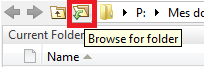
\includegraphics[width=80pt]{../../../img/matlabsimscape/matlab_01} dans le dossier dézippé jusqu'au dossier contenant les fichiers \og .slx \fg\ et \og Simscape \fg,\\
  \begin{center}
  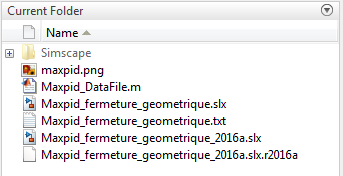
\includegraphics[width=0.4\linewidth]{../../../img/matlabsimscape/matlab_02}
  \end{center}
 \item Faire un clic-droit sur le dossier \og Simscape \fg\ et cliquer sur \og Add to Path \fg,\\
  \begin{center}
  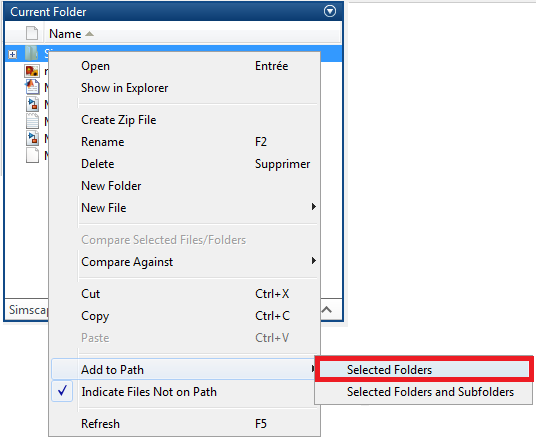
\includegraphics[width=0.4\linewidth]{../../../img/matlabsimscape/matlab_03}
  \end{center}
 \item Double-cliquer sur le fichier correspondant au TP et à la version de Matlab utilisée, il doit avoir une extension en \og slx \fg.\\
  \begin{center}
  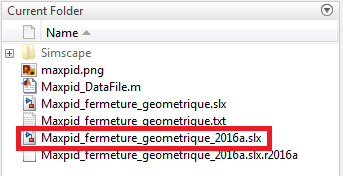
\includegraphics[width=0.4\linewidth]{../../../img/matlabsimscape/matlab_04}
  \end{center}
\end{itemize}
}























% En tête et pied de page
\lhead{\nom}
\rhead{
\includegraphics[width=2cm]{../../../img/logo}}
\lfoot{\auteurs}
\cfoot{Page \thepage}

\fancypagestyle{correction}{%
  \fancyhf{}
  \lhead{\colorbox{danger}{\begin{minipage}{0.65\paperwidth} \textcolor{white}{\textbf{Correction}} \end{minipage}} }
  \rhead{
\includegraphics[width=2cm]{../../../img/logo}}
  \lfoot{Renaud Costadoat}
  \rfoot{\colorbox{danger}{\begin{minipage}{0.6\paperwidth} \begin{flushright}\textcolor{white}{\textbf{Correction}}\end{flushright} \end{minipage}} }}

\renewcommand{\footrulewidth}{0.4pt}

\usepackage{eso-pic}
\newcommand{\BackgroundPic}{%
\put(0,0){%
\parbox[b][\paperheight]{\paperwidth}{%
\vfill
\begin{center}
\hspace{0.5cm}\vspace{0.5cm}

\includegraphics[width=\paperwidth,height=\paperheight,%
keepaspectratio]{../../../img/fond3}%
\end{center}
\vfill
}}}

\newcommand{\BackgroundPicdeux}{%
\put(25,-30){%
\parbox[b][\paperheight]{\paperwidth}{%
\vfill
\begin{center}
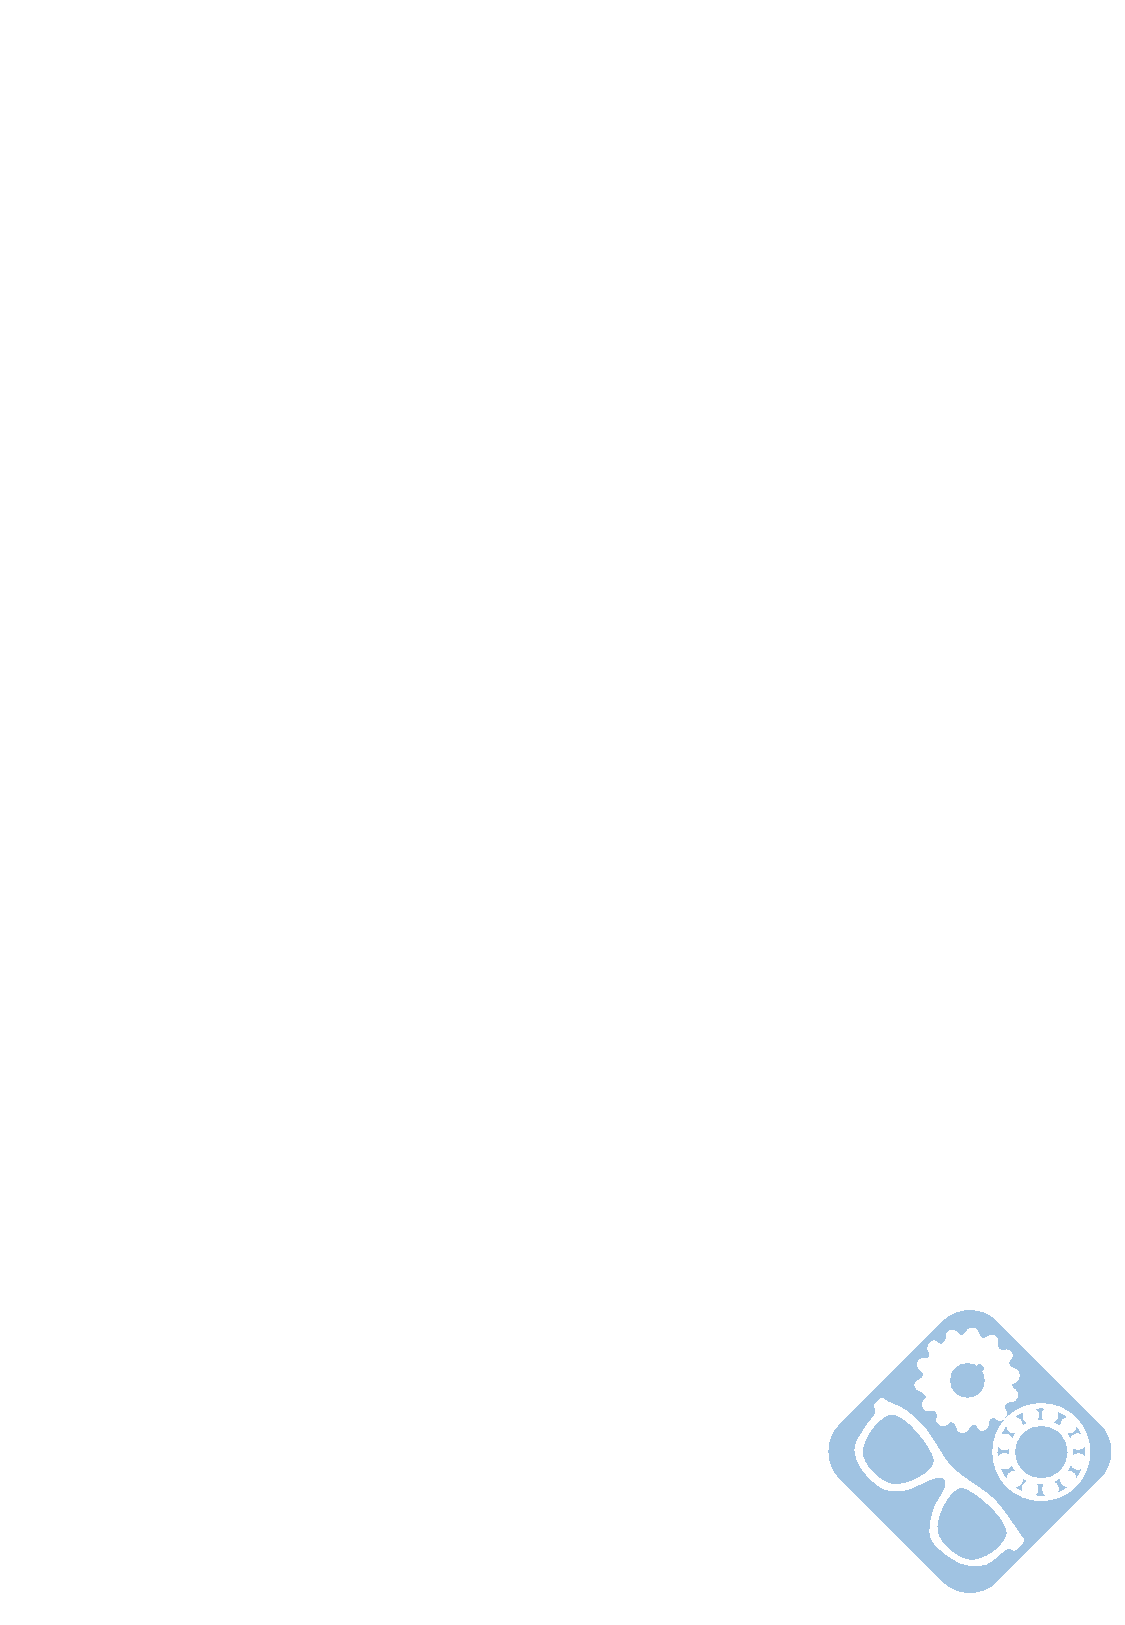
\includegraphics[width=\paperwidth,height=\paperheight,%
keepaspectratio]{../../../img/fond4}%
\end{center}
\vfill
}}}

\newcommand{\activite}[1]{\newpage \cleardoublepage
\renewcommand\arraystretch{2.5}\setcounter{section}{0}\setcounter{subsection}{0}
\ifthenelse{\equal{#1}{1}}{\begin{center}\begin{tabular}{|c|cc p{3cm}|}
\hline
\rowcolor{violt} \supportu & Act & Contenu & Compétences \\\hline
 \multirow{3}{*}{\includegraphics[width=0.2\linewidth]{\supportimageu}} & \begin{LARGE}\textbf{1}\end{LARGE} & \activiteun & \competenceun \\
 & \multicolumn{3}{l|}{Nom: .........................................................................}\\
 & \multicolumn{3}{l|}{Prénom: ....................................................................}\\\hline
\end{tabular}\end{center}}{}
\ifthenelse{\equal{#1}{2}}{\begin{center}\begin{tabular}{|c|cc p{3cm}|}
\hline
\end{tabular}\end{center}}{}}

\begin{document}

\pagestyle{empty}

\vspace*{-3\baselineskip}

\AddToShipoutPicture*{\BackgroundPic}

\ifdef{\auteurdeux}{\begin{tabular}{>{\columncolor{gray!00}}m{.33\linewidth} m{.27\linewidth} >{\columncolor{gray!00}}m{.3\linewidth}}
Séquence \sequence \ - \type \num \ - Îlot \numprint{\ilot} &  \multirow{3}{*}{\hspace{1cm}
\includegraphics[height=1.5cm]{../../../img/logo}} &  \begin{flushright} \multirow{4}{*}{\hspace{1cm}
\includegraphics[height=4cm]{img/qrcode}}\end{flushright}\\
 \textbf{\institute} \\
 \auteurun\\
 \auteurdeux
\end{tabular}}{\begin{tabular}{>{\columncolor{gray!00}}m{.3\linewidth} m{.3\linewidth} >{\columncolor{gray!00}}m{.3\linewidth}}
Séquence \sequence \ - \type \num \ - Îlot \numprint{\ilot}  &  \multirow{3}{*}{\hspace{1cm}
\includegraphics[height=1.5cm]{../../../img/logo}} &  \begin{flushright} \multirow{4}{*}{\hspace{1cm}
\includegraphics[height=4cm]{img/qrcode}}\end{flushright}\\
 \textbf{\institute} \\
 \auteurun
\end{tabular}}

\vspace{1cm}

\begin{center}\colorbox{white}{\huge{\nom}}\end{center}

\vspace{2cm}


\begin{center}\colorbox{white!20}{\includegraphics[height=5cm]{/home/renaud/Documents/Renaud/GitHub/django_education/django_education/static/systemes/\imageun}}\end{center}

\vspace{2cm}



\begin{tabular}{p{.15\linewidth} >{\columncolor{white}}p{.8\linewidth}}
    \rowcolor{gray!20}
    Référence & S\sequence \ - \type\num \ - I\numprint{\ilot} \\
    Compétences & \competences \\
 	\rowcolor{gray!20}
    Description & \descrip \\
    Système & \systemes
  \end{tabular}

\newpage

\AddToShipoutPicture{\BackgroundPicdeux}

\pagestyle{fancy}


\begin{minipage}{0.55\linewidth}
Le winch est un équipement fixé sur le pont ou les mats des voiliers. Il permet d'agir sur les drisses et les écoutes (cordages permettant de hisser une voile) fixées aux angles des voiles. Il intervient principalement au niveau du réglage de la voilure
 \end{minipage}
 \hfill
  \begin{minipage}{0.4\linewidth}
   \centering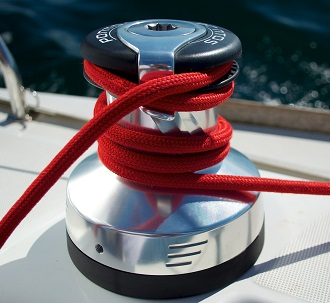
\includegraphics[width=0.7\linewidth]{img/winch.jpg}
  \end{minipage}
 
\section{Activité 1: Modélisation}

\subsection{Action mécanique de contact entre la corde et le tambour}

\begin{minipage}{0.45\linewidth}
Soit une longueur élémentaire de corde $Rd\theta$ en contact avec le Tambour 5 entourant un point M de la zone de contact corde-tambour.

L'étude s'effectue à la limite du glissement.
 \end{minipage}
 \hfill
  \begin{minipage}{0.53\linewidth}
   \centering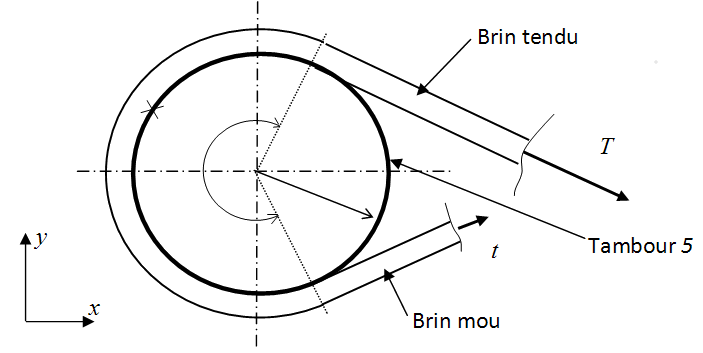
\includegraphics[width=\linewidth]{img/corde_tambour.png}
  \end{minipage}

\begin{center}
	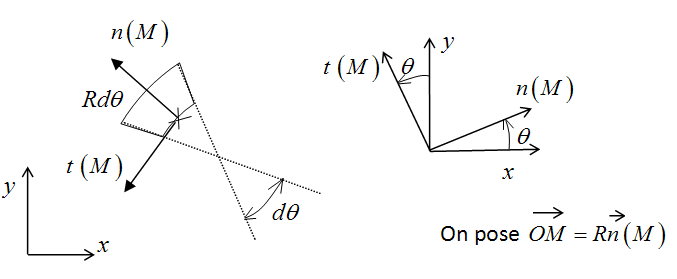
\includegraphics[width=0.7\linewidth]{img/winch_param.png}
\end{center}

 \begin{minipage}{0.45\linewidth}
L'élément de corde précédent est soumis :
\begin{itemize}
 \item à la force élémentaire : $\overrightarrow{df_{T \rightarrow C}(M)}_M$  
 \item à la force élémentaire du brin tendu sur C :  $\overrightarrow{T_{T \rightarrow C}(\theta+d \theta)}_M$  
 \item à la force élémentaire du brin mou sur C : $\overrightarrow{T_{T \rightarrow C}(\theta)}_M$  
\end{itemize}
 \end{minipage}
 \hfill
  \begin{minipage}{0.53\linewidth}
  \centering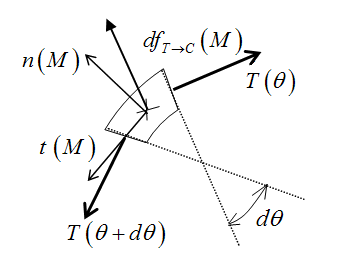
\includegraphics[width=0.7\linewidth]{img/winch_param2.png}
  \end{minipage}


\paragraph{Question 1:} Précisez la normale extérieure matière à la Corde au point M. 

\paragraph{Question 2:} Donnez l'expression de l'aire élémentaire $dS$ de la surface cylindrique de la Corde au point M en fonction de $R$, de $d\theta$ et de la largeur $l$ de la Corde C.

\paragraph{Question 3:} Écrire l'action mécanique locale du Tambour sur la Corde $(T \rightarrow C)$ au point M en fonction du facteur d'adhérence $f_0$ entre le Tambour et la Corde, des vecteurs de la base locale, de la pression de contact $p(\theta)$. (On utilisera la loi de Coulomb relative à l'adhérence à la limite du glissement).

\subsection{Équilibre statique de la corde}

L'équation de résultante du Principe Fondamental de la Statique appliqué à l'élément de corde se traduit par :  

$\overrightarrow{df_{T \rightarrow C}(M)}_M+\overrightarrow{T_{T \rightarrow C}(\theta)}_M+\overrightarrow{T_{T \rightarrow C}(\theta+d \theta)}_M=\overrightarrow{0}$ 

Par projection de l'équation précédente sur la base locale, on en déduit les équations suivantes :
\begin{itemize}
 \item sur $\overrightarrow{n(M)}$: $\overrightarrow{df_{T \rightarrow C}(M)}_M.\overrightarrow{n(M)}-(T_{T \rightarrow C}(\theta)+T_{T \rightarrow C}(\theta+d \theta)).sin\left(\frac{d \theta}{2}\right)=0$ 
 \item sur $\overrightarrow{t(M)}$: $\overrightarrow{df_{T \rightarrow C}(M)}_M.\overrightarrow{t(M)}+(-T_{T \rightarrow C}(\theta)+T_{T \rightarrow C}(\theta+d \theta)).cos\left(\frac{d \theta}{2}\right)=0$ 
\end{itemize}

\paragraph{Question 4:} Linéarisez les expressions précédentes pour $\frac{d \theta}{2} \rightarrow 0$.

\paragraph{Question 5:} Montrez que si l'on pose :

$dT_{T \rightarrow C}(\theta)=T_{T \rightarrow C}(\theta+d \theta)-T_{T \rightarrow C}(\theta)$ et $T_{T \rightarrow C}(\theta)=\frac{T_{T \rightarrow C}(\theta+d \theta)+T_{T \rightarrow C}(\theta)}{2}$, on obtient :

\begin{itemize}
 \item sur $\overrightarrow{n(M)}$: $\overrightarrow{df_{T \rightarrow C}(M)}_M.\overrightarrow{n(M)}=T_{T \rightarrow C}(\theta).d \theta$ 
 \item sur $\overrightarrow{t(M)}$: $\overrightarrow{df_{T \rightarrow C}(M)}_M.\overrightarrow{t(M)}=-dT_{T \rightarrow C}(\theta)$ 
\end{itemize}

\paragraph{Question 6:} En remplaçant $\overrightarrow{df_{T \rightarrow C}(M)}_M$ par son expression (question 5), montrez que :

\begin{itemize}
 \item sur $\overrightarrow{n(M)}$: $T_{T \rightarrow C}(\theta)=p(\theta).Rl$,
 \item sur $\overrightarrow{t(M)}$: $dT_{T \rightarrow C}(\theta)=-p(\theta).f_0.Rld \theta$ 
\end{itemize}



\paragraph{Question 7:} Écrivez le rapport $\frac{dT_{T \rightarrow C}}{T_{T \rightarrow C}}(\theta)$ et simplifiez son expression.



\paragraph{Question 8:} Intégrez le rapport $\frac{dT_{T \rightarrow C}}{T_{T \rightarrow C}}(\theta)$ entre $\theta=0$ et $\theta=\theta_f$.



\paragraph{Question 9:} En remplaçant $T_{T \rightarrow C}(0)=T$ et $T_{T \rightarrow C}(\theta_f)=t$, donnez l'expression de $t$ en fonction de $T$.



\paragraph{Question 10:} En déduire, à l'aide des résultats de l'étude expérimentale la valeur moyenne du facteur d'adhérence entre la corde et le tambour. 



\paragraph{Question 11:} Tracez, avec cette valeur du facteur d'adhérence, la courbe théorique sur le graphique issu de l'expérimentation du Q2. 



On souhaite maintenant déterminer le couple transmis par le Tambour 5 à la Corde.

\paragraph{Question 12:} Déterminez le moment élémentaire $\overrightarrow{dM_{O,T \rightarrow C}}(\theta)$ au point O du Tambour sur la Corde en fonction de $T_{T \rightarrow C}(\theta)$ et R, à l'aide des questions 5 et 8.



\paragraph{Question 13:} Intégrez le moment élémentaire $\overrightarrow{dM_{O,T \rightarrow C}}(\theta)$ entre $\theta=0$ et $\theta=\theta_f$. En déduire le moment en O : $\overrightarrow{M_{O,T \rightarrow C}}$.



\paragraph{Question 14:} Calculez la valeur de la norme de ce moment pour 1, 2 et 3 tours d'enroulement de la corde.



\paragraph{Question 15:} Estimez l'intensité de la force exercée par l'utilisateur.



\cleardoublepage

\section{Activité 2: Étude expérimentale}

 \begin{minipage}{0.45\linewidth}
Soit le montage expérimental suivant.

Soit $t$ l'effort dans le brin mou et $T$ l'effort dans le brin tendu. La corde est immobile par rapport au tambour (adhérence).
 \end{minipage}
 \hfill
  \begin{minipage}{0.53\linewidth}
   \centering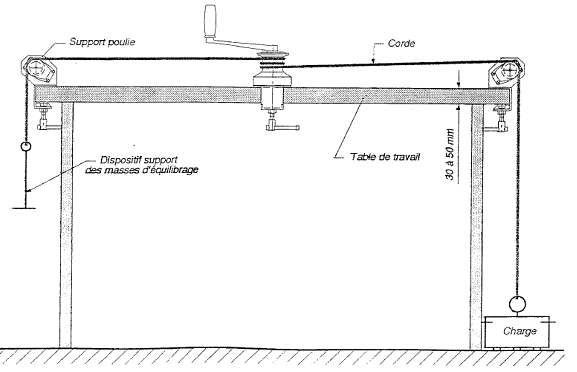
\includegraphics[width=0.9\linewidth]{img/winch_exp.png}
  \end{minipage}

\begin{enumerate}
 \item Enrouler la corde autour du tambour (1, 2 ou 3 tours),
 \item Suspendre la charge et les masses d'équilibrage pour que l'ensemble soit en équilibre,
 \item Diminuez progressivement l'effort $t$ (en enlevant des masses d'équilibrage) et relever la valeur pour laquelle l'adhérence n'existe plus.
\end{enumerate}

\paragraph{Question 1:} Remplissez le tableau de mesure suivant:

\begin{center}
\begin{tabular}{|c|c|c|c|}
\hline
Nombre de tours & t(N) 1er essai & t(N) 2ème essai & t(N) moyen \\
\hline
1 & & & \\
\hline
2 & & & \\
\hline
3 & & & \\
\hline
\end{tabular}
\end{center}

\paragraph{Question 2:} Placez les points expérimentaux de $t$ en fonction de l'angle d'enroulement $\theta$ sur un graphique.



\end{document}
